%**************************************************************
\subsubsection{Package it.tecsen.smacs.model}
\label{subsubsec:it-tecsen-smacs-model}

\begin{figure}[!h]
  \centering 
  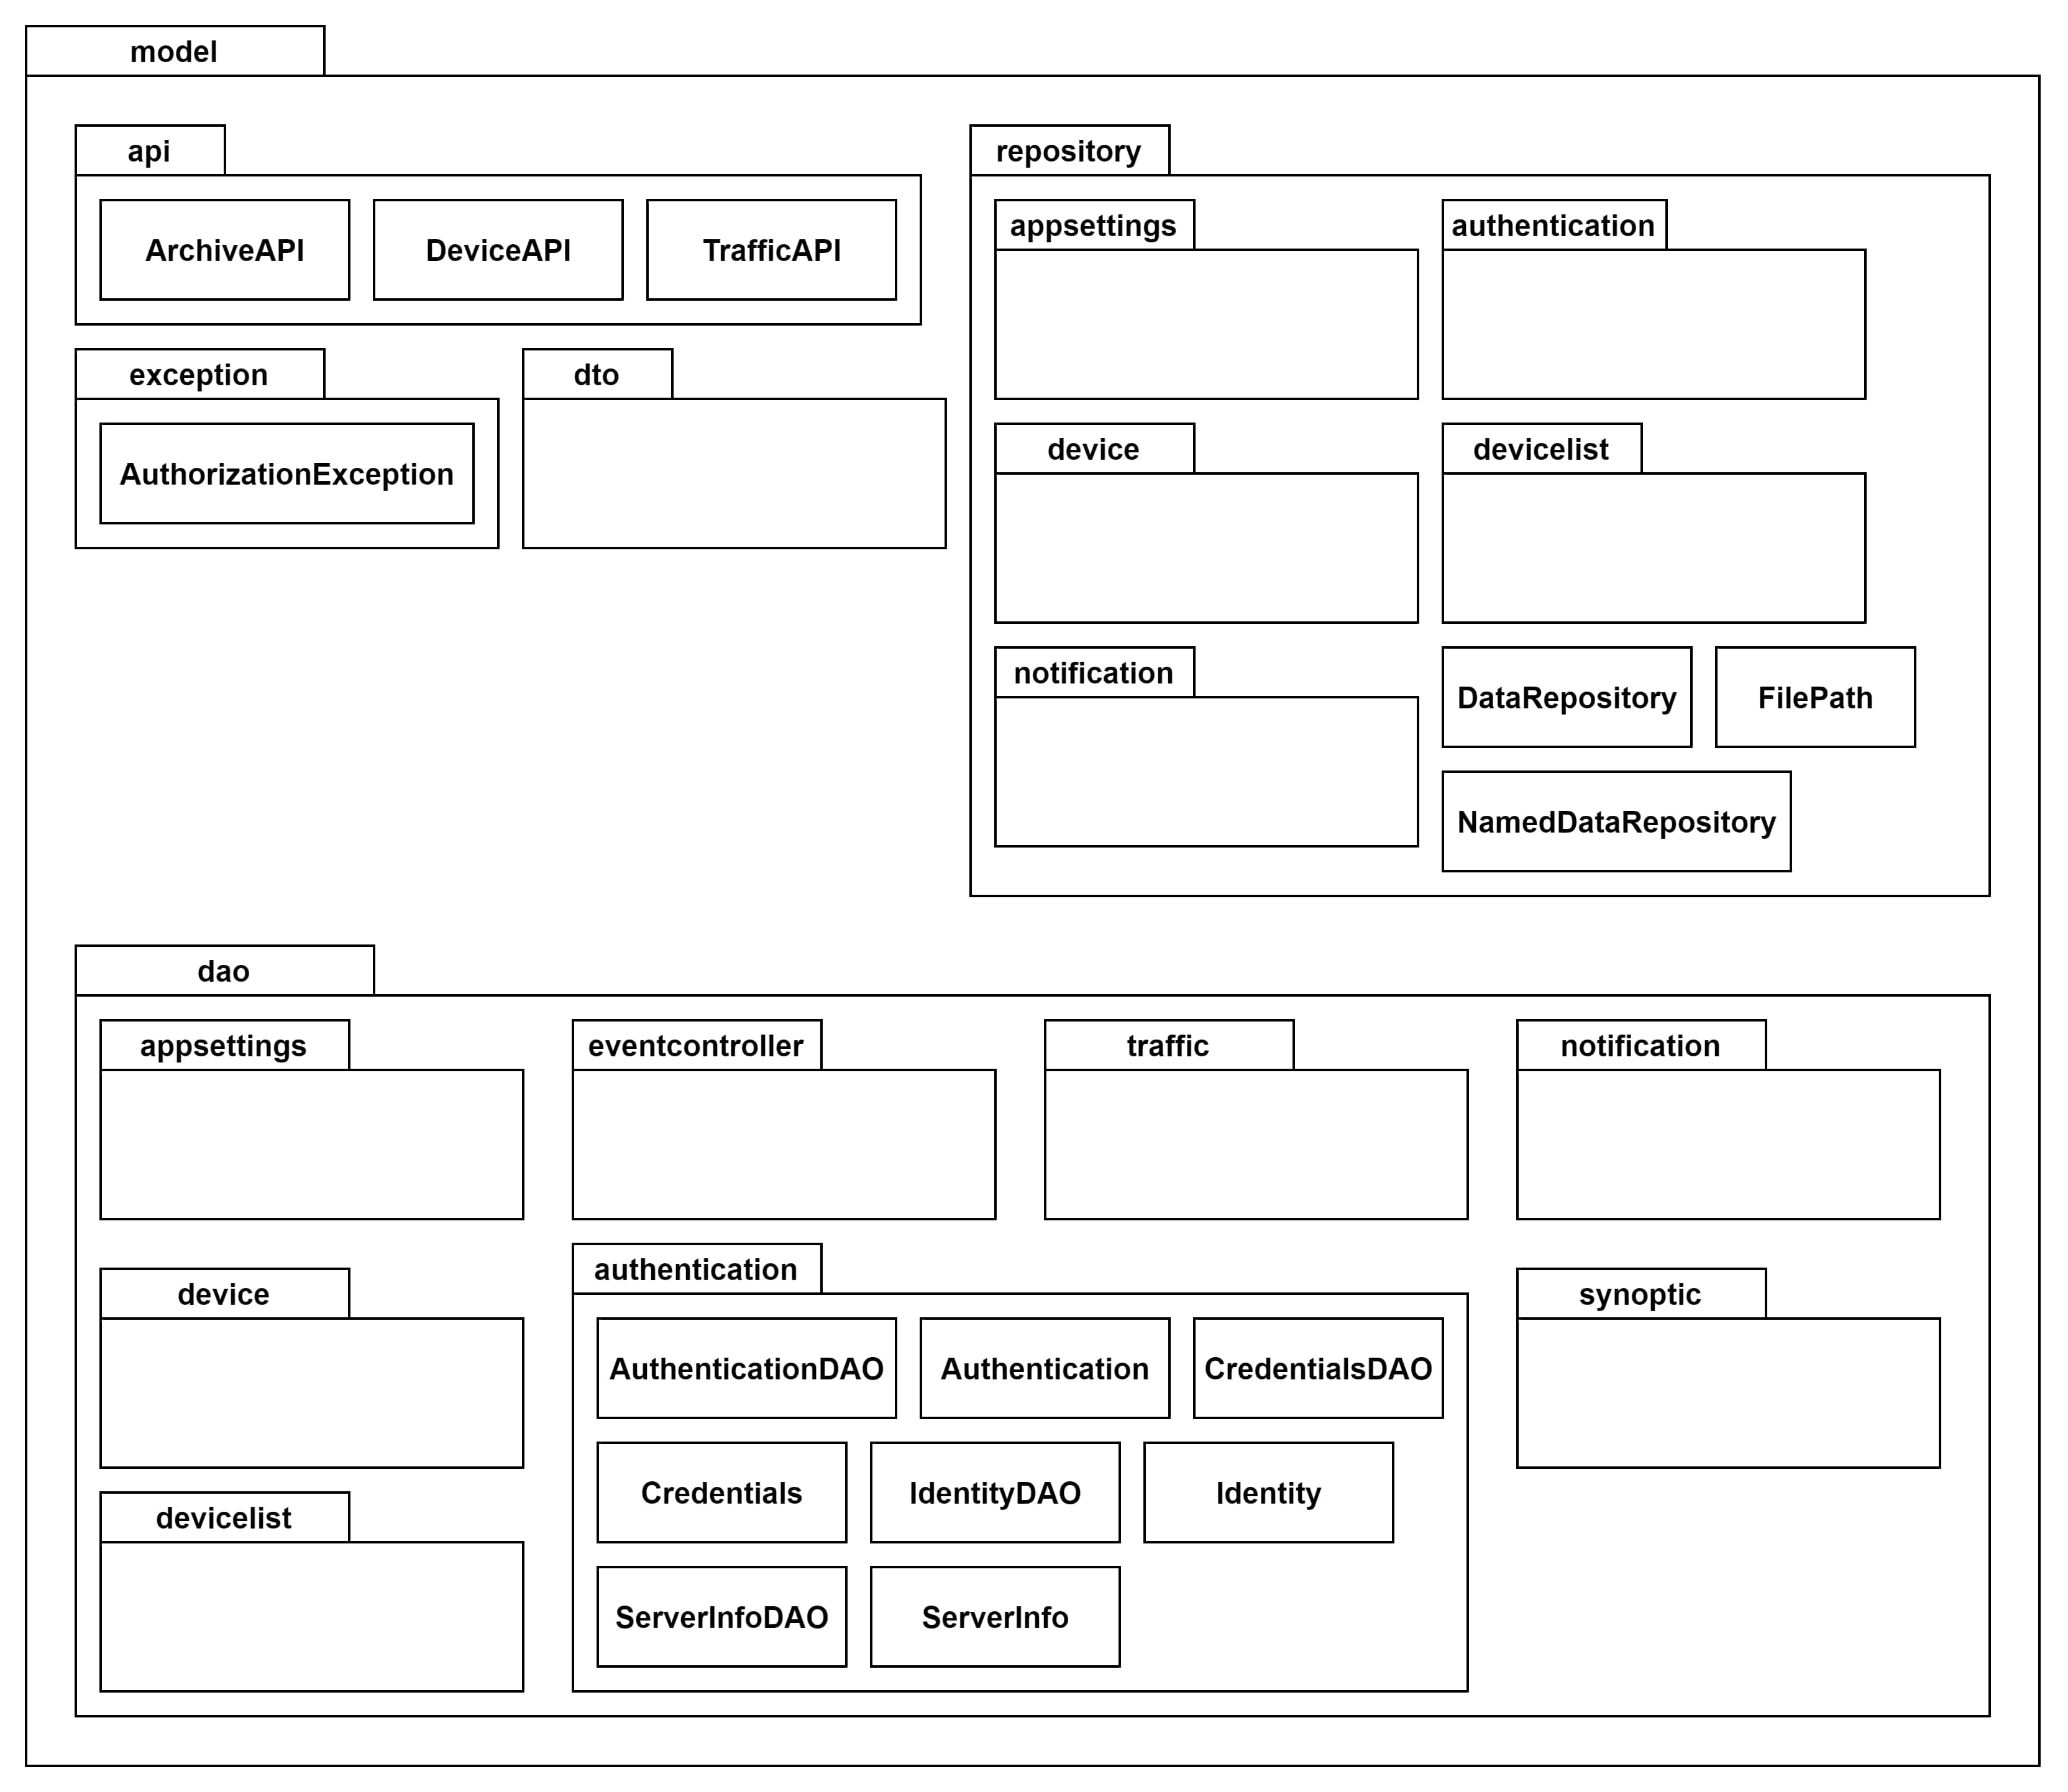
\includegraphics[width=1.0\columnwidth]{capitolo-6/organizzazione-package/model} 
  \caption{Diagramma del package \texttt{it.tecsen.smacs.model}}
\end{figure}
Questo package implementa il modello dell'applicazione.\\
Si può dividere in più aree con compiti specifici, rappresentate dai sotto-package:
\begin{itemize}
  \item \texttt{api} contiene classi che utilizzano il wrapper del package \texttt{webserviceclient} per interrogare le \gls{restg} e ritornare il risultato sotto forma di \gls{dto};
  \item \texttt{exception} contiene eccezioni che possono essere generate dalle classi presenti in questo package;
  \item \texttt{repository} contiene interfacce e classi per memorizzare su supporto persistente (le implementazioni usano dei file come supporto persistente) i dati ricevuti dai \gls{dao};
  \item \texttt{dao} contiene tutti le classi \gls{dao} che sono necessarie ai membri del package \texttt{viewmodel} per funzionare. Utilizza i package \texttt{api} e \texttt{repository} per ottenere i dati da ritornare sotto forma di \gls{dto};
  \item \texttt{dto} contiene tutti le classi \gls{dto} che sono necessarie al funzionamento dei package \texttt{api}, \texttt{dao} e \texttt{viewmodel}.
\end{itemize}
Sebbene \texttt{api} e \texttt{dao} ritornino entrambi \gls{dto}, c'è una differenza:
\begin{itemize}
  \item il primo non fa nessuna elaborazione sui dati, semplicemente li ottiene dalle \gls{restg} sotto forma di \gls{json}, ne fa il parsing e restituisce quanto ottenuto;
  \item il secondo elabora i \gls{dto} ottenuti dal primo e li ritorna elaborati (per fare un esempio, una lista ricevuta da \texttt{api} potrebbe essere ordinata, filtrata e poi ritornata).
\end{itemize}